\documentclass{book}
\usepackage{graphicx}
\usepackage[explicit]{titlesec}
\usepackage{xcolor}
\usepackage{lipsum}% just to generate text
\usepackage{multirow}
\usepackage{booktabs}
%\colorlet{myrulecolor}{black}
\definecolor{myrulecolor}{RGB}{150,20,0}% define the color for the rules

\titleformat{\chapter}[display]
  {\normalfont\scshape\Huge}
  {\hspace*{-70pt}\thechapter.~#1}
  {-15pt}
  {\hspace*{-110pt}{\color{myrulecolor}\rule{\dimexpr\textwidth+80pt\relax}{3pt}}\Huge}
\titleformat{name=\chapter,numberless}[display]
  {\normalfont\scshape\Huge}
  {\hspace*{-70pt}#1}
  {-15pt}
  {\hspace*{-110pt}{\color{myrulecolor}\rule{\dimexpr\textwidth+80pt\relax}{3pt}}\Huge}
\titlespacing*{\chapter}{0pt}{0pt}{30pt}

\begin{document}
\chapter*{27. Estimating Abundance\\
          \noindent{\large{Chris Sutherland \& J. Andrew  Royle}}}

\section*{1. Introduction}
%intro: motivate CMR

Fundamental to much of applied ecology, including species management
and conservation, is the ability to reliably estimate population size,
or $abundance$. This is particularly true for reptiles given growing
evidence of declines globally (Gibbons et al. 2000, Reading et
al. 2010) and high levels of data deficiency (B{\"o}hm et a.l 2013). The
major challenge arises because rarely are all the individuals in a
population encountered during a survey, and that the
resulting $counts$, i.e. the number of individuals encountered, $n$,
represents only some fraction of the true abundance, $N$. Although the
distinction between counts and true abundance is an important one, the
two are intuitively related and, by repeatedly sampling and marking
individuals in a population, capture-recapture methods provide a
formalization of this relationship and a framework for estimating true
population size.

In this chapter, we provide a non-technical overview of `closed
population capture-recapture' models, a class of well established
models that are widely applied in ecology (Borchers et al. 2002,
Williams et al. 2001), and regularly adopted for studies of reptiles
(Mazerolle et al. 2007), to estimate abundance from counts of marked
individuals while accounting for imperfect detection. We first describe
some classic closed population models for estimating abundance (Otis
et al., 1978), then consider some recent extensions that provide a
spatial context for the estimation of abundance, and therefore
density, $D$ (spatial or spatially-explicit capture-recapture: Efford
2004, Royle et al. 2014), and finally provide an example of estimating
abundance and density of reptiles using an artificial cover object
survey of slow worms, \textit{Anguis fragilis}.

\subsection*{2. Closed Population Capture-Recapture}
\subsubsection*{2.1. Sampling a population}
%A typical CMR study

The primary objective in a closed population capture-recapture study
is to estimate the abundance of a population of interest. The
population of $N$ individuals is subjected to repeated sampling for a
specified number of occasions, say $K$, where, in the first sampling
occasion, all captured individuals are marked an released, and then at
each subsequent sampling occasion the detection of marked individuals
is recorded and unmarked individuals are marked. Identifying a focal
population, the spatial extent of the population is implicitly defined
and the method of capture depends on the species in question and
available resources. For reptiles, survey methods that allow
individuals to be captured and marked include, for example, visual
searches within a defined area (Zylstra et al. 2010), cage traps
(Tyrrell et al. 2009, Christy et al. 2010) or pitfall traps, and the
use of artificial cover objects (ACO, Grant et al. 1992) (see also
Chapter X).  Once captured, individuals can be uniquely identified
using either natural markings that can be used to determine individual
identity (Sacchi et al. 2010), using tags or markings (Grant \&
Doherty 2007) or physical marking such as toe clipping (Paulissen \&
Meyer 2000) (see also Chapter X).

Such repeated sampling results in individual encounter histories that,
for each of the $i=1,\ldots,n$ individuals encountered, describes
whether or not individuals were detected in each of the $K$
occasions. For example, in a $K = 4$ occasion capture-recapture study,
an individual with an encounter $y_i = (0 1 0 1)$ was encountered
$\hbox{y}_i = 2$ times; first in occasion 2, and then again in
occasion 4, and was not encountered in occasions one or three. In
Table \ref{enchist} we provide an example of encounter history data
for a $K=4$ occasion capture-recapture study during which $n=8$
individuals were captured.

\begin{table}[h]
  \centering
  \caption{An example of an encounter history for a $K = 4$ occasion capture-recapture study during which $n=8$ individuals were detected.}
  \label{enchist}
 \begin{tabular}{lccccr}
 \toprule
    &\multicolumn{5}{c}{Occasion} \\
  Individual & 1 & 2 & 3 & 4 & y\\
 \midrule
  1   & 0 & 1 & 0 & 1 & 2 \\
  2   & 1 & 0 & 0 & 1 & 2 \\
  3   & 0 & 1 & 1 & 1 & 3 \\
  4   & 1 & 1 & 0 & 0 & 2 \\
  5   & 1 & 0 & 0 & 1 & 2 \\
  6   & 0 & 0 & 1 & 1 & 2 \\
  7   & 0 & 0 & 1 & 0 & 1 \\
  n=8 & 1 & 0 & 0 & 1 & 2 \\
 \bottomrule
 \end{tabular}
\end{table}

Estimating abundance using encounter history data collected using the
general sampling scheme we have described above is basically the
process of estimating how many individuals were $missed$, i.e., how
many individuals have encounter history $\hbox{y}_i = 0$. The ability
to do so requires that the following basic assumptions are met:

\begin{enumerate}
\item the population is closed to demographic processes and to
  movement
\item individual marks can be identified unambiguously and are not lost
\item individuals are equally likely to be captured
\end{enumerate}

A `closed' population is one that experiences no additions or
subtractions for the duration of the study, and whose size is
therefore assumed to be fixed during sampling. Defining a sampling
period over which the assumption of closure can be satisfied means
that an individual detected at least once during the study was present
for the entire study, and therefore, failure to detect that individual
in any occasion was due to imperfect detection. This highlights the
importance of the second assumption -- that individuals are identified
unambiguously -- because misidentification would lead to erroneous
encounter histories that don't reflect the true process of
encountering individuals. The third assumption is less important as we
will see later, but satisfying this assumption means that we can employ
the simplest formulation of a capture-recapture model, model $M_0$.

\subsubsection*{2.2. Estimating abundance using model $M_0$}

Under model $M_0$, the encounter probability for each individual,
$p_i$, is assumed to be the same for all individuals in the
population, i.e., $p_i = p$. Then, whether or not we encounter an
individual $i=1,2,\ldots,N$ during sampling occasion $k$, $y_{ik}$, is
a Bernoulli trial (a ``coin flip'') with constant probability $p$,
which we can write formally as:
\[
y_{ik} \sim \hbox{Bernoulli}(p).
\]
i.e., there are no individual or temporal covariates that affect
$p$. The basic idea of all closed population capture-recapture methods
is that the pattern of detections in the encounter histories of
individuals observed at least once provides information about
individual detectability, or detection probability, $p$, which in
turn, can be used to estimate the number of individuals $not$
encountered.  The underlying concept can be understood by recognizing
that the observed number of individuals $n$ is related to the total
population size $N$ by the expression:
\[
 E(n) = N\tilde{p}
\]
where $E()$ denotes statistical expectation and $\tilde{p}$ is the
probability that an individual is captured {\it at all} during the
study. In a study of $K$ survey occasions $\tilde{p}$ is directly
related to the basic parameter $p$ by the formula
\[
 \tilde{p} = 1-(1-p)^K
\]
This expression applies to model $M_0$ but the
 expression relating $p$ to $\tilde{p}$ is different depending on
the specific  capture-recapture model being considered.
In general the parameter $p$ can be estimated from the observed
encounter histories and, in turn, this is used to estimate $\tilde{p}$
and then finally we estimate $N$ by $\hat{N} = n/\tilde{p}$.

This estimator of $N$ is typically called the `conditional estimator' of $N$
because the quantity $\tilde{p}$ is the probability of capture in at
least 1 occasion, and the likelihood is formally constructed by
conditioning on the event that an individual is encountered at all
(i.e., at least once).  The conditional estimator of population size
$N$ has only one canonical estimated parameter, that being $p$, and
$N$ is a derived parameter. An alternative framework for inference
about $N$ is based on the `full likelihood' in which $N$ appears
explicitly in the likelihood.  The two approaches are both widely used
in all contexts, and there is little practical difference.



\subsubsection*{2.3. Variation in $p$: beyond $M_0$}

The assumption of equal capture probability is a rather restricting
one and there are many situations under which the capture
probabilities would be expected to vary. For these situations, model
$M_0$ is not appropriate although and Otis et al. (1978) described a
family of models that can be used to deal with most sources of
variation in individual encounter probabilities:
\begin{itemize}
\item[$M_0$] Capture probability is the same for all individuals (Section 2.2)
\item[$M_t$] Capture probability is the same for all individuals, but
  varies between sampling occasions (\textbf{t}ime) (note that below we use
  $k$ for the time index in our development).
\item[$M_b$] Capture probabilities vary depending on whether or not
  individuals have been captured previously (\textbf{b}ehavioral
  response).
\item[$M_h$] Capture probabilities vary among individuals (individual
  \textbf{h}eterogeneity).
\end{itemize}

Variations of these different models exist. For example, the usual
application of model $M_t$ involves occasion-specific parameters
$p_{k}$, but we can also consider systematic variation in detection
probability that results from explicit covariates. For example, we
could model seasonal variation in $p_k$ using a quadratic polynomial
in Julian day, $J_{k}$, such as:
\[
 logit(p_{k}) = \alpha_0 + \alpha_1 J_{k} + \alpha_2 J^{2}_{k}
\]
and estimate the parameters $\alpha_0$, $\alpha_1$ and $\alpha_2$
instead of fully occasion specific parameters $p_k$.  The behavioral
response model is usually parameterized as a permanent change in $p$
for individuals subsequent to their initial capture (i.e. $p_{pre}$
and $p_{post}$, for capture probability {\it prior to} and {\it after}
first capture respectively). This could be the result of `trap
happiness' due to having baited traps (uncommon in reptile studies) or
it could be the result of `trap shyness' due to aversion to
handling. Sometimes a transient or ephemeral behavioral response may
be sensible (Yang and Chao 2005). Under this type of model the
response to initial capture only lasts for a brief period after
initial capture.

Model $M_h$ has been an important model in capture-recapture because
it has long been recognized that the existence of individual
heterogeneity in capture probability will lead to under-estimation of
$N$ when it is not accounted for.  Thus much attention has been
focused on developing more flexible classes of model $M_h$.  Thus,
model $M_h$, has many different variations. Norris and Pollock (1996)
formulated the model in terms of a finite mixture or latent class
model in which each individual in the population belongs to a finite
(and small) number of classes represented by distinct values of $p$
(see also Pledger 2000). Dorazio and Royle (2003) considered
continuous mixtures such as the beta-binomial and logit-normal models
(see also Coull and Agresti 1999).

\subsubsection*{2.4. Removal Sampling}

Removal sampling is unlike other capture-``recapture'' methods in the
sense that individuals are captured only once but then removed from
the population and, hence, not available to be recaptured. The idea of
removal sampling is that by repeatedly removing individuals, we should
realize a decrease in catch frequency, and this realized decrease is
informative about detection probability which can then be used to
obtain an estimate of the population size $N$ as it was {\it prior} to
the initiation of the sampling activity. Intuitively, we expect to
capture $p \times N$ individuals during a single sample and, if we
remove those individuals, we should expect to capture capture $p
(N - p N) = p(1-p) N$ individuals in the 2nd bout of
removal sampling. Note that the ratio of these two removal counts is
$1-p$ which produces a direct estimate of $p$ from which $N$ can be
estimated by a suitable algebraic function of the counts.

In practice, removal sampling is done using `temporary' removals in
which an area is searched and individuals are temporarily housed in a
bucket or cage during successive passes (Garden et al. 2007). At the
end of the study they would normally be released to where they were
initially captured. Of course earlier applications of removal sampling
to fisheries involved permanent removal, typically harvest, but that
is not practical in most studies of reptiles.

\subsubsection*{2.5. Hierarchical capture-recapture models}

Closed population models are usually described in the context of
sampling a single closed population. However, in practice, it is
almost always the case that multiple populations of individuals are
sampled. For example, small mammal trapping studies might involve a
number of live trapping grids, or reptile and amphibian studies might
involve a number of distinct cover board arrays.  In such cases we can
think of the distinct populations being sampled by each array as spatial strata,
with potentially stratum specific parameters such as $p_{g}$, $N_{g}$
($g$ for 'grid') which could be estimated by applying closed
population models to data collected from each stratum.  However,
analyzing the data from these stratified populations ``one-at-a-time''
can be statistically inefficient (Converse and Royle 2012). Instead,
there can be distinct advantages to combining all of the data into a
single capture-recapture model but tying the different models together
by imposing model structure on the detection probability or abundance
parameters using a hierarchical modeling framework.  For example, a
simple model allowing for variation in population size among a
collection of $g=1,2,\ldots,G$ trap arrays is $N_{g} \sim
\mbox{Poisson}(\lambda)$. This model allows each population to have
it's own `size' but builds in a weak stochastic dependence between the
populations, so that all of the data are used to estimate the shared
parameter $\lambda$. The end result is more precision to estimate the
population-specific parameters by combining the information from all
of the distinct populations. See Royle (2004), Dorazio et al. (2005)
and Royle, Converse and Link (2012).


\subsection*{2.5 Individual covariate models and distance sampling}

Model $M_h$ is the standard closed population model when {\it
  unexplained} individual heterogeneity in capture-probability
exists. However an important related class of models are models in
which individual heterogeneity can be explained by explicit individual
covariates. These are often called ``individual covariate models''
but, in keeping with the classical nomenclature on closed population
models, K\'{e}ry and Schaub (2012) referred to these models as ``model
$M_{x}$'', the $x$ representing some explicit covariate (of course
multiple covariates are allowed).  Classical examples of covariates
influencing detection probability are type of animal (juvenile/adult
or male/female), a continuous covariate such as body mass, or a
discrete covariate such as group or cluster size. For example, in
models of aerial survey data, it is natural to model the detection
probability of a group as a function of the observation-level
individual covariate, ``group size'' (Royle 2009, Langtimm et
al. 2011).

The basic encounter model for model $M_x$ is the same as our other
closed models, the Bernoulli encounter model:
\[
y_{i} \sim \mbox{Bernoulli}(p_{i}).
\]
To model the covariate, we use a logit model for encounter probability
of the form:
\begin{equation}
 \mbox{logit}(p_{i}) = \alpha_0 + \alpha_1 x_{i}
\end{equation}
where $x_i$ is the covariate value for individual $i$ and the
parameters $\alpha_0$ and $\alpha_1$ are the parameters to be
estimated.

Traditionally, estimation of $N$ in model $M_{x}$ is achieved using
methods based on ideas of unequal probability sampling (i.e.,
Horvitz-Thompson estimation). This idea was developed independently by
Huggins (1989) and Alho (1990). The estimator of $N$ is given as a
derived parameter:
\[
\hat{N} = \sum_{i=1}^{n} \frac{1}{\tilde{p}_{i}}
\]
where $\tilde{p}_{i}$ is the probability that individual $i$ appeared
in the sample.  This is related to the more fundamental parameters
$\alpha$ in the model for detection probability according to:
\[
\tilde{p}_{i}  = 1- (1-p_{i})^K
\]
where $p_{i}$ is a function of parameters $\alpha_{0}$ and
$\alpha_{1}$.  In practice, parameters are estimated from the
conditional-likelihood of the observed encounter histories.

An alternative formulation of model $M_x$ is the ``full likelihood''
which requires that we put a model on the individual covariate $x$
allowing for the sample not only of the encounter histories but also
of the covariate to be extrapolated to the population.  For example,
if we have a continuous trait measured on each individual, then we
might assume that $x$ has a normal distribution:
\[
x_{i} \sim \mbox{Normal}(\mu,\sigma^{2})
\]
If the covariate was group size then, naturally, some discrete
probability mass function would be needed. Inference for individual
covariate models from the standpoint of the  full likelihood is
discussed widely, including in Royle (2009), K\'{e}ry and Schaub (2012).

Individual covariate models are important in practice for the simple
reason that heterogeneity exists in almost every capture-recapture
study due to the spatial organization of traps and of individuals in
the population (see next section). Thus, they were adopted historically
to account for spatial structure in capture-recapture (Boulanger and
McLellan 2001, Karanth and Nichols 1998).  For this purpose an
individual covariate is created which describes {\it where} the
individual is located in relation to the trapping array.  This
approach leads naturally to more recent spatial capture-recapture
models described in the next section.

A very important and popular method for
estimating abundance is distance sampling (Buckland et
al. 2005). Unlike capture-recapture sampling, distance sampling
requires only a single ``snap-shot'' sample of the population. For
each detected individual distance from the observer is
measured. Information about detection probability comes from an
assumed model for the relationship between detection probability and
distance to observer. Distance sampling is, formally, a special case
of individual covariate models where there is only a single replicate
sample ($K=1$), and the individual covariate is distance.

\subsection*{3. Spatial Capture-Recapture}

One of the main deficiencies with classical closed population models
is that they do not permit direct estimation of animal $density$
because, in almost all practical field applications, it is not
possible to precisely define the area sampled by a set of trapping
devices. This is because individuals being captured move about space
and can be captured without the biologists knowing from whence those
individuals originated or how much space they are using. Newly
developed {\it spatial capture-recapture} (SCR) models (also called
spatially-explicit capture-recapture, SECR) provide a technical
framework for dealing with this problem (Efford 2004, Borchers and
Efford 2008, Royle and Young 2008, Royle et al. 2014). These models
follow logically on from model M$_x$, where $x$ is the activity center
of the individual as we will see below.

The sampling scheme for a $spatial$ capture-recapture analysis is the
same as described above, i.e., there is a population of $N$
individuals, but now we consider each individual having an activity
center that has $X$ and $Y$ coordinates
($\textbf{s}_i=[s_{i,X},s_{i,Y}]$). Now the goal is to estimate the
number of individuals (or activity centers) within a region of
interest which we refer to as a $state$-$space$, or ${\cal S}$, which
is to say we wish to estimate density: $D = N/||{\cal S}||$, where
$||{\cal S}||$ is the area of ${\cal S}$. We assume that these
activity centers are distributed uniformly throughout across space:
\[
\textbf{s}_i \sim \hbox{Uniform}({\cal S}).
\]
As before, the population is subjected to sampling using some trapping
devices (for convenience, we will refer to these as `traps'). However,
we explicitly acknowledge both how many traps there are: $j=1,...,J$
traps, and the locations of each of the traps, which we denote as
$x_j$.  The acknowledgment of the spatial structure of the traps
means observations can be spatially indexed so encounter histories
describe $who$ ($i$), $when$ ($k$), and importantly, $where$ ($j$)
individuals were located, i.e., $y_{i,j,k}$. Typically, these
observations are assumed to be Bernoulli outcomes:
\[
y_{i,j,k} \sim \hbox{Bernoulli}(p_{i,j,k}),
\]
where $p_{i,j,k}$ is the probability of encountering individual $i$ in
trap $j$, and occasion $k$, which at a minimum depends on the distance between the trap location
($x_j$) and the individuals activity center ($s_i$) as follows:
\begin{equation}
p_{i,j} = p_0 \times e^{-(1/2\sigma^2) \hbox{d}(x_{j},s_{i})^{2}}.
\end{equation}
(it may also depend on sample occasion $k$ in some fashion).
This is refereed to as the half-normal  encounter
model where $\hbox{logit}(p_0) = \alpha_0$ is the baseline encounter
probability, which is the probability of encountering an individual at
its' activity center, the parameter $\sigma$ describes the rate at
which detection probability declines as a function of distance, and
$\hbox{d}(x_{j},s_{i})$ is the Euclidean distance between trap $j$ and
the activity center of individual $i$. In a spatial capture-recapture
analysis, the parameters to be estimated are $\alpha_0$ and $\sigma$
in addition to population size $N$.  As in model $M_h$, the additional
parameter $\sigma$ accommodates individual heterogeneity in $p$ but,
unlike model $M_h$, the parameter represents an explicit source of
heterogeneity, that due to distance between individual activity or
home range centers and trap locations.

SCR models address the density estimation problem directly by
parameterizing the model directly in terms of individual activity
centers $s_i$ and prescribing the state-space ${\cal S}$. The
inference problem then reduces to estimating the number of such
activity centers in the well-defined area ${\cal S}$, i.e., density.
Density, $D$, is simply a transformation of $N$: $D =
N/\mbox{Area}({\cal S})$.

\subsection*{4. Software}

Non-spatial closed population capture-recapture models can be fit
using both classical (frequentist) and Bayesian methods, and here we
outline some of the common software options and material sources for
doing so.

By far the most widely used software for fitting such models is the
Windows-based program {\bf MARK} (White \& Burnham 1999), a free, user
friendly and extremely well-documented application for fitting most of
the standard closed population models using maximum likelihood
(www.phidot.org/software/mark). In an effort to facilitate easier
model development, increased reproducibility and to allow for a more
organized and automated work flow, Laake \& Rexstad (2008) developed
the {\bf R} package {\tt RMark}, an interface between {\bf R} and {\bf
  MARK} that can be used to construct input files and extract output
that can manipulated in the {\tt R} environment
(\verb|www.phidot.org/software/mark/rmark/|). The {\bf R} package {\tt
  unmarked} (Fiske \& Chandler 2011)
can also be used to fit hierarchical versions of some
standard closed population capture-recapture models using maximum
likelihood (see K\'{e}ry and Royle 2015, ch. 7).
In addition to detailed
documentation, both {\bf MARK} (\verb|www.phidot.org/forum/index.php|) and
{\tt unmarked}
(\verb|https://groups.google.com/forum/#!forum/unmarked|) have
supporting web based forums.

Spatial capture-recapture models cannot (yet) be implemented in {\bf
  MARK}, and, although a windows-based spatial equivalent exists ({\bf
  DENSITY}: Efford, et al. 2004), it is no longer in development and
likelihood analysis of SCR models is typically conducted using the
{\bf R} package {\tt secr} (Efford 2011). {\tt secr} implements a wide
variety of spatial capture-recapture methods, including spatial
version of the models described above and in Otis et al. (1978), all
within the {\bf R} environment ({\tt secr} forum can be found here:
\verb|https://groups.google.com/forum/#!fo| \verb|rum/secrgroup|)

Often situations arise when an analysis requires a `non-standard' approach (e.g. an integrated population model: Schaub \& Abadi 2011, demographic metapopulation models: Sutherland et al. 2014, models for transience and dispersal: Royle et al. {\it In review}). In these cases, available likelihood-based methods cannot be used and instead a Bayesian analysis is preferred. Bayesian methods, specifically the use of Markov chain Monte Carlo (MCMC) using the {\tt BUGS} language, offer a great deal of flexibility and modeling freedom (K\'{e}ry and Schaub 2013).

Bayesian analysis of capture-recapture models is done using a method
related to classical ``data augmentation'' from the statistics
literature (e.g., Tanner \& Wong, 1987).  This is a general concept in
statistics but, in the context of capture-recapture models, where $N$
is unknown, it has a consistent implementation across classes of
capture-recapture models and one that is really convenient from the
standpoint of doing MCMC (Royle et al. 2007; Royle \& Dorazio
2012). Chapter 6 of K\'{e}ry \& Schaub (2011) provide an accessible and
complementary development of Bayesian analysis of non-spatial closed
population models. The tremendous benefit of formulating SCR models in
the {\tt BUGS} language is that it is relatively trivial to extend
form the the non-spatial model to the formulation on the closed
population model. In their book, Royle et al. (2014) provide a
thorough treatment of SCR and Bayesian methods for
analyzing a SCR models which has an associated forum
(\verb|https://groups.google.com/forum/#!forum/spati| \verb|alcapturerecapture|).

\subsection*{5. Slow worm example}

We provide an example here using a study of the slow worm (Anguis
fragilis) conducted in Mueterschwanderberg, canton Nidwalden,
Switzerland (Meier 2012, thesis). A more detailed SCR analysis of the
data from that study is given by Meier et al. (in prep). Here we
analyze a portion of the data from one of the artificial cover object
arrays which used 23 cover objects (Fig. \ref{fig.fig1}). This ACO
array was operated over 59 days and it produced encounter histories on
44 unique individuals, 23 captured once, 4 capture twice, 4 thrice, 5
four times, 3 five times, 1 six times and 4 seven times.

\begin{figure}[h]
\centering
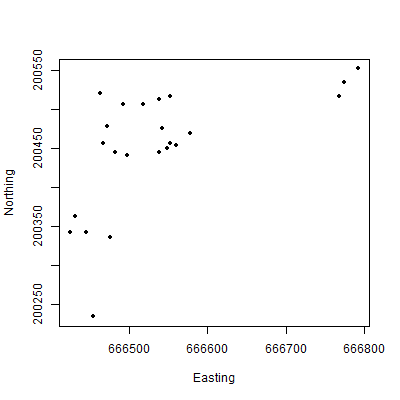
\includegraphics[height=4in,width=4in]{traps.png}
\caption{
Artificial cover object (ACO) array from the slow worm study of Meier
2012).  Sampling from this array over 59 days produced encounter
histories of 44 individuals.
}
\label{fig.fig1}
\end{figure}

An immediately obvious `feature' of this ACO array is the irregular
and uneven distribution of cover objects.  While we may apply
capture-recapture models to the data from this study to estimate
population size $N$, it is clear that the irregular ACO array should
be a hindrance to a clear interpretation of this estimate because
there is no obvious way to compute a sample area for this
grid. Moreover, the spatial heterogeneity in trap density is almost
certain to induce heterogeneity in detection probability of
individuals depending on the location of individuals relative to
traps. While we can use model $M_h$ to account for some heterogeneity,
that model is not an explicit model of heterogeneity due to spatial
proximity of individuals to traps. Nevertheless, we fit both models
$M_0$ and $M_h$ to these data in order to see how they compare.  We
will also fit the SCR model to see how we can convert an estimate of
$N$ to density.

We fit the logit-normal variety of model $M_h$ (Coull and Agresti
1999, Dorazio and Royle 2003) which assumes that the
logit-transformation of individual detection probability $p_i$ has a
normal distribution with variance $\theta^2$:
\[
 logit(p_i) \sim \mbox{Normal}(\mu, \theta^2).
\]
Therefore this model has 3 parameters ($N$, $\mu$ and $\theta$).  The
additional parameter $\theta$ accommodates over-dispersion or
individual heterogeneity in $p$.
For the analysis of the SCR model we defined
 the state-space by creating the minimum area rectangle around the trap array
and then buffering that by 40 meters, creating a state-space having an
area of 10.64 ha (Figure 1).
The summary results from fitting these 3 models to the slow worm data
are given in Table \ref{tab.results}. We note that
AIC is {\it not} comparable between SCR and ordinary closed models because the
models are fitted to different data sets:
SCR models use the individual, trap and occasion-specific
encounter data whereas ordinary capture-recapture models aggregate
over all traps to produce a simpler reduced-information individual by
occasion-specific encounter history.  A key point of this comparison
is that the estimates of $n_0$ (the number of uncaptured individuals),
and hence of $N$, are radically different. Model $M_h$ and the SCR
model both accommodate heterogeneity in encounter probability which is
indicated in these data ($\theta = 1.114$ under the logit-normal model
$M_h$, which is favored strongly over model $M_0$ by AIC). Thus, the estimated $N$ is increased substantially in
comparison to model $M_0$. In addition, the SCR model produces an
estimate of $N$ that applies to a specific, well-defined region (the
state-space) having an area of 10.64 ha. Thus we can compute directly
an estimate of the {\it density} of slow worms, which comes out to
14.68 slow worms/ha.  With model $M_0$ and model $M_h$ there's really
no telling what area should be associated with those estimates, and
therefore no basis for comparison with the estimate obtained by the
SCR model.


\begin{table}[ht]
\centering
\caption{The results of fitting models M0 and Mh and an ordinary SCR
  model to the slow worm data. Model $M_h$ has one extra parameter
  compared to model $M_0$, the individual heterogeneity parameter
  $\theta$. The SCR model has one additional parameter, $\sigma$, the
  scale parameter of the encounter probability model relating
  individual $p$ to distance between individual activity center and
  trap location. }
\begin{tabular}{crrrrrr}
\toprule
Model & $p$ or $p_0$ &  $n_0$   & extra parameter & N      & D(/ha)  & AIC     \\
\midrule
M0    &  0.0396      & 3.97     &                 & 47.97  &         & -73.42  \\
Mh    &  0.0149      & 30.88    & 1.114           & 74.88  &         & -89.21  \\
SCR   &  0.0501      & 112.14   & 21.005          & 156.14 & 14.68   & 320.39  \\
\bottomrule
\end{tabular}
\label{tab.results}
\end{table}

\section*{6. Summary}

Capture-recapture methods have been the standard for estimating population size and density for many decades and provide a framework for sampling populations and estimating key parameters, namely population size or abundance. However, we have also argued that capture-recapture is inherently spatial because of the way we typically conduct sampling (e.g. artificial cover objects, pitfall or cage traps etc...), and yet traditionally this has almost never been addressed in the application of capture-recapture methods. These non-spatial methods have a number of deficiencies that would appear to limit their usefulness in practice (but, strangely, have not). For example, they do not allow the direct estimation of density, they do not account for the spatial organization of trapping arrays, or of individuals within the population being studied. Moreover, despite capture-recapture studies often involving
explicit questions about spatial ecology, space is largely ignored, opting instead for a ``fishbowl'' view of systems.

We demonstrated that the source of heterogeneity that is likely to be an issue an almost all CR studies, i.e., spatial distribution of individuals relative to traps, can be address using spatial extensions of capture-recapture models, namely ``spatial capture-recapture''. The obvious benefit of SCR is that the spatial region for which abundance is estimated is explicitly defined and that \textit{absolute} density can be computed directly. Perhaps of greater importance however, is the explicit focus on the spatial processes giving rise to encounter data which enables researchers to study many aspects of spatial ecology from individual encounter history data, including resource selection or space usage (Royle et al. 2013), landscape connectivity (Royle et al. 2013b; Sutherland et al. 2014), spatial variation in density (Borchers and Efford 2008, Royle et al. 2013), and movement or dispersal (Schaub and Royle 2014, Ergon and Gardner 2014, Royle et al. {\it in review}).

As has been discussed in detail throughout this book, reptiles represent an important component of many communities, are a group of animals in global decline, and can be extremely difficult to monitor. Many of the methods described in earlier chapters for monitoring, capturing and identifying individuals for reptilian populations lend themselves naturally to analysis using capture-recapture methods and should be preferred over indices of abundance like raw counts. Moreover, many of these sampling procedures are naturally spatial (trapping grids, line transect etc...) in which case we recommend analysis using spatial capture recapture methods in order to arrive at meaningful, spatial referenced abundance estimates as we demonstrated with the slow worms example.



\section*{Literature Cited}
\newcommand{\rf}{\vskip .1in\par\sloppy\hangindent=1pc\hangafter=1
             \noindent}

\rf Alho, J. M. (1990). Logistic regression in capture-recapture models. \textit{Biometrics}, 623-635.

\rf B{\"o}hm, M., Collen, B., Baillie, J. E., Bowles, P., Chanson, J., Cox, N., \& Cheylan, M. (2013). The conservation status of the world’s reptiles. \textit{Biological Conservation}, 157, 372-385.

\rf Borchers, D. L., , Buckland, S. T.  and W. Zucchini. 2002. Estimating animal abundance: closed populations (Vol. 13). Springer Science \& Business Media.

\rf Borchers, D.L. and M.G. Efford. 2008. Spatially explicit maximum likelihood methods for capture-recapture studies. {\it Biometrics} 64, 377-385.

\rf Boulanger, J., \& McLellan, B. (2001). Closure violation in DNA-based mark-recapture estimation of grizzly bear populations. \textit{Canadian Journal of Zoology}, 79(4), 642-651.

\rf Buckland, S. T., Anderson, D. R., Burnham, K. P., \& Laake, J. L. (2005). Distance sampling. John Wiley \& Sons, Ltd.

\rf Cagle, F. R. (1939). A system of marking turtles for future identification. \textit{Copeia}, 1939(3), 170-173.

\rf Christy, M. T., A. A. Yackel, Adams, G H. Rodda, J. A. Savidge, and C. L. Tyrrell. Modelling detection probabilities to evaluate management and control tools for an invasive species. \textit{Journal of Applied Ecology} 47, no. 1 (2010): 106-113.

\rf Coull, B. A., \& Agresti, A. (1999). The Use of Mixed Logit Models to Reflect Heterogeneity in Capture-Recapture Studies. \textit{Biometrics}, 55(1), 294-301.

\rf Converse, S. J., \& Royle, J. A. (2012). Dealing with incomplete and variable detectability in multi-year, multi-site monitoring of ecological populations. Design and Analysis of Long-term Ecological Monitoring Studies. Cambridge University Press, Cambridge, UK, 426-442.

\rf Dorazio, R. M., \& Royle, J. A. (2003). Mixture models for estimating the size of a closed population when capture rates vary among individuals. \textit{Biometrics}, 59(2), 351-364.

\rf Dorazio, R. M., Jelks, H. L., \& Jordan, F. (2005). Improving Removal-Based Estimates of Abundance by Sampling a Population of Spatially Distinct Subpopulations. \textit{Biometrics}, 61(4), 1093-1101.

\rf Efford, M. 2004. Density estimation in live-trapping studies. {\it Oikos}  106, 598-610.

\rf Efford, M. G., Dawson, D. K., \& Robbins, C. S. (2004). DENSITY: software for analysing capture-recapture data from passive detector arrays. \textit{Animal Biodiversity and Conservation}, 27(1), 217-228.

\rf Ergon, T., \& Gardner, B. (2014). Separating mortality and emigration: modelling space use, dispersal and survival with robust-design spatial capture-recapture data. \textit{Methods in Ecology and Evolution}, 5(12), 1327-1336.

\rf Efford, M. G. (2011). secr: Spatially explicit capture-recapture models. R package version, 2(0).

\rf Fiske, I., \& Chandler, R. B. (2011). unmarked: An R package for fitting hierarchical models of wildlife occurrence and abundance. \textit{Journal of Statistical Software}, 43(10), 1-23.

\rf Garden, J.G., McAlpine, C.A., Possingham, H.P., and Jones, D.N. (2007) Using multiple survey methods to detect terrestrial reptiles and mammals: what are the most successful and cost-efficient combinations?. \textit{Wildlife Research} 34, 218-227.

\rf Gibbons, et al. (2000). The Global Decline of Reptiles, Déjà Vu Amphibians Reptile species are declining on a global scale. Six significant threats to reptile populations are habitat loss and degradation, introduced invasive species, environmental pollution, disease, unsustainable use, and global climate change. \textit{BioScience}, 50(8), 653-666.

\rf Grant, B. W., A. D. Tucker, J. E. Lovich, A. M. Mills, P. M. Dixon, and J. W. Gibbons. (1992). The use of coverboards in estimating patters of repile and amphibian biodiversity. Wildlife 2001: Populations 379-403.

\rf Grant, T. J. \& Doherty, P. F. (2007). Monitoring of the Flat-Tailed Horned Lizard With Methods Incorporating Detection Probability. \textit{The Journal of wildlife management}, 71(4), 1050-1056.

\rf Huggins, R. M. (1989). On the statistical analysis of capture experiments. \textit{Biometrika}, 76(1), 133-140.

\rf  Karanth, K. U., \& Nichols, J. D. (1998). Estimation of tiger densities in India using photographic captures and recaptures. \textit{Ecology}, 79(8), 2852-2862.

\rf K\'{e}ry, M., \& Schaub, M. (2012). Bayesian population analysis using WinBUGS: a hierarchical perspective. Academic Press.

\rf K\'{e}ry, M., \& Royle, J. A. (2015). Applied Hierarchical Models. Academic Press.

\rf Laake, J., \& Rexstad, E. (2008). RMark: an alternative approach to building linear models in MARK. Program MARK: a gentle introduction.

\rf Langtimm, C. A., Dorazio, R. M., Stith, B. M., \& Doyle, T. J. (2011). New aerial survey and hierarchical model to estimate manatee abundance. \textit{The Journal of Wildlife Management}, 75(2), 399-412.

\rf Mazerolle, M. J., Bailey, L. L., Kendall, W. L., Andrew Royle, J., Converse, S. J., \& Nichols, J. D. (2007). Making great leaps forward: accounting for detectability in herpetological field studies. \textit{Journal of Herpetology}, 41(4), 672-689.

\rf Meier, A. (2012). Reptilienaufwertungskonzept am Mueterschwandenberg. Bachelorarbeit. Zurich University of Applied Sciences, Wädenswil. 74 pp.

\rf Norris III, J. L., \& Pollock, K. H. (1996). Nonparametric MLE under two closed capture-recapture models with heterogeneity. \textit{Biometrics}, 639-649.

\rf Otis, D. L., Burnham, K. P., White, G. C., \& Anderson, D. R. (1978). Statistical inference from capture data on closed animal populations. \textit{Wildlife monographs}, 3-135.

\rf Paulissen, M. A., \& Meyer, H. A. (2000). The effect of toe-clipping on the gecko Hemidactylus turcicus. \textit{Journal of Herpetology}, 282-285.

\rf Pledger, S. (2000). Unified maximum likelihood estimates for closed capture-recapture models using mixtures. \textit{Biometrics}, 56(2), 434-442.

\rf R Development Core Team. (2004). R: A language and environment for statistical computing. R Foundation for Statistical Computing Vienna, Austria.

\rf Reading, C. J., L. M. Luiselli, G. C. Akani, Xavier Bonnet, G. Amori, Jean-Marie Ballouard, E. Filippi, Guy Naulleau, D. Pearson, \& L. Rugiero. (2010). Are snake populations in widespread decline?. \textit{Biology Letters}, 6, 777-780.

\rf Royle, J. A. (2004). Generalized estimators of avian abundance from count survey data. \textit{Animal Biodiversity and Conservation}, 27(1), 375-386.

\rf Royle, J.A., R.M. Dorazio and W.A. Link. (2007). Analysis of multinomial models with unknown index using data augmentation. {\it Journal of Computational and Graphical Statistics}  16, 67-85.

\rf Royle, J.A. and K.V. Young. (2008). A hierarchical model for spatial capture-recapture data. {\it Ecology}  89, 2281-2289.

\rf Royle, J. A. (2009). Analysis of capture-recapture models with individual covariates using data augmentation. {\it Biometrics}, 65(1), 267-274.

\rf Royle, J. A., Converse, S. J., \& Link, W. A. (2012). Data Augmentation for Hierarchical Capture-recapture Models. arXiv preprint arXiv:1211.5706.

\rf Royle, J. A. and R. M. Dorazio. 2012. Parameter-expanded data augmentation for Bayesian analysis of capture-recapture models. {\it Journal of Ornithology} 152(2), 521-537.

\rf Royle, J. A., Chandler, R. B., Gazenski, K. D., \& Graves, T. A. (2013). Spatial capture-recapture models for jointly estimating population density and landscape connectivity. \textit{Ecology}, 94(2), 287-294.

\rf Royle, J. A., R. B. Chandler, C. C. Sun, and A. K. Fuller. (2013). Integrating resource selection information with spatial capture-recapture. {\it Methods in Ecology and Evolution} 4(6), 520-530.

\rf Royle, J. A., R. B. Chandler, R. Sollmann and B. Gardner. (2014). Spatial Capture-Recapture. Academic Press.

\rf Royle, J. A., Fuller, A. K., and Sutherland, C. (in
review). Spatial capture-recapture models allowing for Markovian
transience or dispersal. {\it Population Ecology}.

\rf Sacchi, R., Scali, S., Pellitteri-Rosa, D., Pupin, F., Gentilli, A., Tettamanti, S. \& Fasola, M. (2010). Photographic identification in reptiles: a matter of scales. \textit{Amphibia-Reptilia}, 31(4), 489-502.

\rf Schaub, M., \& Abadi, F. (2011). Integrated population models: a novel analysis framework for deeper insights into population dynamics. \textit{Journal of Ornithology}, 152(1), 227-237.

\rf Schaub, M., \& Royle, J. A. (2014). Estimating true instead of apparent survival using spatial Cormack-Jolly-Seber models. \textit{Methods in Ecology and Evolution}, 5(12), 1316-1326.

\rf Sutherland, C. S., Elston, D. A., \& Lambin, X. (2014). A demographic, spatially explicit patch occupancy model of metapopulation dynamics and persistence. \textit{Ecology}, 95(11), 3149-3160.

\rf Sutherland, C., A. K. Fuller and J. A. Royle. (2015). Modelling non-Euclidean movement and landscape connectivity in highly structured ecological networks. {\it Methods in Ecology and Evolution}  6, 169-177.

\rf Tanner, M. A., \& Wong, W. H. (1987). The calculation of posterior distributions by data augmentation. \textit{Journal of the American statistical Association}, 82(398), 528-540.

\rf Tyrrell, C. L., Christy, M. T., Rodda, G. H., Yackel Adams, A. A., Ellingson, A. R., Savidge, J. A., Dean-Bradley, K., \& Bischof, R. (2009). Evaluation of trap capture in a geographically closed population of brown treesnakes on Guam. \textit{Journal of Applied Ecology}, 46(1), 128-135.

\rf Williams, B. K., Nichols, J. D., \& Conroy, M. J. (2002). Analysis and management of animal populations. Academic Press.

\rf Yang, H. C., \& Chao, A. (2005). Modeling animals' behavioral response by Markov chain models for capture-recapture experiments. \textit{Biometrics}, 61(4), 1010-1017.

\rf Zylstra, Erin R., Robert J. Steidl, and Don E. Swann. Evaluating survey methods for monitoring a rare vertebrate, the Sonoran desert tortoise. \textit{The Journal of Wildlife Management}, 74.6 (2010): 1311-1318.

\end{document}


